\protect\hyperlink{main-nav}{≡} \protect\hyperlink{close-nav}{×}

\hypertarget{section-1.8-logarithmic-functions}{%
\section{Section 1.8: Logarithmic
Functions}\label{section-1.8-logarithmic-functions}}

Logarithms are the inverse of exponential functions -- they allow us to
undo exponential functions and solve for the exponent. They are also
commonly used to express quantities that vary widely in size.

\hypertarget{logarithm-equivalent-to-an-exponential}{%
\paragraph{Logarithm Equivalent to an
Exponential}\label{logarithm-equivalent-to-an-exponential}}

The logarithm (base \textbackslash{}(b\textbackslash{})) function,
written \textbackslash{}( \textbackslash{}log\_b (x) \textbackslash{}),
is the inverse of the exponential function (base
\textbackslash{}(b\textbackslash{})), \textbackslash{}( b\^{}x
\textbackslash{}).

This means the statement \textbackslash{}( b\^{}a=c \textbackslash{}) is
equivalent to the statement \textbackslash{}( \textbackslash{}log\_b
(c)=a \textbackslash{}).

\hypertarget{properties-of-logs-inverse-properties}{%
\paragraph{Properties of Logs: Inverse
Properties}\label{properties-of-logs-inverse-properties}}

\begin{itemize}
\tightlist
\item
  \textbackslash{}( \textbackslash{}log\_b(b\^{}x)=x \textbackslash{})
\item
  \textbackslash{}( b\^{}\{\textbackslash{}log\_b(x)\}=x
  \textbackslash{})
\end{itemize}

To view this video please enable JavaScript, and consider upgrading to a
web browser that \href{http://videojs.com/html5-video-support/}{supports
HTML5 video}

\hypertarget{example-1}{%
\paragraph{Example 1}\label{example-1}}

Write these exponential equations as logarithmic equations:

\begin{enumerate}
\tightlist
\item
  \textbackslash{}( 2\^{}3=8 \textbackslash{})
\item
  \textbackslash{}( 5\^{}2=25 \textbackslash{})
\item
  \textbackslash{}(10\^{}\{-4\}=\textbackslash{}frac\{1\}\{10000\}\textbackslash{})
\end{enumerate}

\begin{enumerate}
\tightlist
\item
  \textbackslash{}( 2\^{}3=8 \textbackslash{}) is equivalent to
  \textbackslash{}( \textbackslash{}log\_2(8)=3 \textbackslash{}).
\item
  \textbackslash{}( 5\^{}2=25 \textbackslash{}) is equivalent to
  \textbackslash{}( \textbackslash{}log\_5(25)=2 \textbackslash{}).
\item
  \textbackslash{}(10\^{}\{-4\}=\textbackslash{}frac\{1\}\{10000\}\textbackslash{})
  is equivalent to \textbackslash{}(
  \textbackslash{}log\_\{10\}\textbackslash{}left(\textbackslash{}frac\{1\}\{10000\}\textbackslash{}right)=-4
  \textbackslash{}).
\end{enumerate}

\hypertarget{example-2}{%
\paragraph{Example 2}\label{example-2}}

Solve \textbackslash{}( 2\^{}x=10 \textbackslash{}) for
\textbackslash{}(x\textbackslash{}).

By rewriting this expression as a logarithm, we get \textbackslash{}(
x=\textbackslash{}log\_2(10) \textbackslash{}).

To view this video please enable JavaScript, and consider upgrading to a
web browser that \href{http://videojs.com/html5-video-support/}{supports
HTML5 video}

While this does define a solution, and an exact solution at that, you
may find it somewhat unsatisfying since it is difficult to compare this
expression to the decimal estimate we made earlier. Also, giving an
exact expression for a solution is not always useful--often we really
need a decimal approximation to the solution. Luckily, this is a task
calculators and computers are quite adept at. Unluckily for us, most
calculators and computers will only evaluate logarithms of two bases.
Happily, this ends up not being a problem, as we'll see briefly.

\hypertarget{common-and-natural-logarithms}{%
\paragraph{Common and Natural
Logarithms}\label{common-and-natural-logarithms}}

The \textbf{common log} is the logarithm with base 10, and is typically
written \textbackslash{}( \textbackslash{}log(x) \textbackslash{}).

The \textbf{natural log} is the logarithm with base
\textbackslash{}(e\textbackslash{}), and is typically written
\textbackslash{}( \textbackslash{}ln(x) \textbackslash{}).

\hypertarget{example-3}{%
\paragraph{Example 3}\label{example-3}}

Evaluate \textbackslash{}( \textbackslash{}log(1000) \textbackslash{})
using the definition of the common log.

To evaluate \textbackslash{}( \textbackslash{}log(1000)
\textbackslash{}), we can say \textbackslash{}(
x=\textbackslash{}log(1000) \textbackslash{}), then rewrite into
exponential form using the common log base of 10:\textbackslash{}{[}
10\^{}x=1000. \textbackslash{}{]}

From this, we might recognize that 1000 is the cube of 10, so
\textbackslash{}(x = 3\textbackslash{}).

We also can use the inverse property of logs to write \textbackslash{}(
log\_\{10\}\textbackslash{}left(10\^{}3\textbackslash{}right) =3
\textbackslash{}).

\begin{longtable}[]{@{}lll@{}}
\caption{Values of the common log}\tabularnewline
\toprule
\endhead
Number & Number as exponential & log(number)\tabularnewline
1000 & \textbackslash{}( 10\^{}3 \textbackslash{}) & 3\tabularnewline
100 & \textbackslash{}( 10\^{}2 \textbackslash{}) & 2\tabularnewline
10 & \textbackslash{}( 10\^{}1 \textbackslash{}) & 1\tabularnewline
1 & \textbackslash{}( 10\^{}0 \textbackslash{}) & 0\tabularnewline
0.1 & \textbackslash{}( 10\^{}\{-1\} \textbackslash{}) &
-1\tabularnewline
0.01 & \textbackslash{}( 10\^{}\{-2\} \textbackslash{}) &
-2\tabularnewline
0.001 & \textbackslash{}( 10\^{}\{-3\} \textbackslash{}) &
-3\tabularnewline
\bottomrule
\end{longtable}

\hypertarget{example-4}{%
\paragraph{Example 4}\label{example-4}}

Evaluate \textbackslash{}( \textbackslash{}log(500) \textbackslash{})
using you calculator or computer.

Using a computer or calculator, we can evaluate and find that
\textbackslash{}( \textbackslash{}log(500)\textbackslash{}approx 2.69897
\textbackslash{}).

Another property provides the basis for solving exponential equations.

\hypertarget{properties-of-logs-exponent-property}{%
\paragraph{Properties of Logs: Exponent
Property}\label{properties-of-logs-exponent-property}}

\textbackslash{}(
\textbackslash{}log\_b\textbackslash{}left(A\^{}r\textbackslash{}right)=r\textbackslash{},\textbackslash{}log\_b(A)
\textbackslash{})

\hypertarget{solving-exponential-equations}{%
\paragraph{Solving exponential
equations:}\label{solving-exponential-equations}}

\begin{enumerate}
\tightlist
\item
  Isolate the exponential expressions when possible.
\item
  Take the logarithm of both sides.
\item
  Utilize the exponent property for logarithms to pull the variable out
  of the exponent.
\item
  Use algebra to solve for the variable.
\end{enumerate}

To view this video please enable JavaScript, and consider upgrading to a
web browser that \href{http://videojs.com/html5-video-support/}{supports
HTML5 video}

\hypertarget{example-5}{%
\paragraph{Example 5}\label{example-5}}

In the last section, we predicted the population (in billions) of India
\textbackslash{}(t\textbackslash{}) years after 2008 by using the
function \textbackslash{}( f(t)=1.14(1+0.0134)\^{}t \textbackslash{}).
If the population continues following this trend, when will the
population reach 2 billion?

We need to solve for the \textbackslash{}(t\textbackslash{}) so that
\textbackslash{}(f(t) = 2\textbackslash{})

\begin{longtable}[]{@{}ll@{}}
\toprule
\endhead
\textbackslash{}(2=1.14(1.0134)\^{}t\textbackslash{}) & Initial
equation.\tabularnewline
\textbackslash{}(\textbackslash{}dfrac\{2\}\{1.14\}=1.0134\^{}t\textbackslash{})
& Divide by 1.14 to isolate the exponential expression.\tabularnewline
\textbackslash{}(\textbackslash{}ln\textbackslash{}left(\textbackslash{}dfrac\{2\}\{1.14\}\textbackslash{}right)=\textbackslash{}ln\textbackslash{}left(1.0134\^{}t\textbackslash{}right)\textbackslash{})
& Take the logarithm of both sides of the equation.\tabularnewline
\textbackslash{}(\textbackslash{}ln\textbackslash{}left(\textbackslash{}dfrac\{2\}\{1.14\}\textbackslash{}right)=t\textbackslash{},\textbackslash{}ln(1.0134)\textbackslash{})
& Apply the exponent property on the right side.\tabularnewline
\textbackslash{}( t =
\textbackslash{}dfrac\{\textbackslash{}ln\textbackslash{}left(\textbackslash{}dfrac\{2\}\{1.14\}\textbackslash{}right)\}\{\textbackslash{}ln(1.0134)\}\textbackslash{})
& Divide both sides by
\textbackslash{}(\textbackslash{}ln(1.0134)\textbackslash{})\tabularnewline
\textbackslash{}( t\textbackslash{}approx 42.23 \textbackslash{}text\{
years\} \textbackslash{}) &\tabularnewline
\bottomrule
\end{longtable}

If this growth rate continues, the model predicts the population of
India will reach 2 billion about 42 years after 2008, or approximately
in the year 2050.

\hypertarget{example-6}{%
\paragraph{Example 6}\label{example-6}}

Solve \textbackslash{}( 5e\^{}\{-0.3t\}=2 \textbackslash{}) for
\textbackslash{}( t \textbackslash{}).

First we divide by 5 to isolate the exponential: \textbackslash{}{[}
e\^{}\{-0.3t\}=\textbackslash{}frac\{2\}\{5\}. \textbackslash{}{]}

Since this equation involves \textbackslash{}(e\textbackslash{}), it
makes sense to use the natural log:

\begin{longtable}[]{@{}ll@{}}
\toprule
\endhead
\textbackslash{}(\textbackslash{}ln\textbackslash{}left(e\^{}\{-0.3t\}\textbackslash{}right)=\textbackslash{}ln\textbackslash{}left(\textbackslash{}dfrac\{2\}\{5\}\textbackslash{}right)\textbackslash{})
& Take the natural log of both sides.\tabularnewline
\textbackslash{}(-0.3t=\textbackslash{}ln\textbackslash{}left(\textbackslash{}dfrac\{2\}\{5\}\textbackslash{}right)\textbackslash{})
& Utilizing the inverse property for logs.\tabularnewline
\textbackslash{}( t =
\textbackslash{}dfrac\{\textbackslash{}ln\textbackslash{}left(\textbackslash{}dfrac\{2\}\{5\}\textbackslash{}right)\}\{-0.3\}\textbackslash{})
& Now dividing by -0.3.\tabularnewline
\textbackslash{}( t\textbackslash{}approx 3.054 \textbackslash{})
&\tabularnewline
\bottomrule
\end{longtable}

In addition to solving exponential equations, logarithmic expressions
are common in many physical situations.

\hypertarget{example-7}{%
\paragraph{Example 7}\label{example-7}}

In chemistry, pH is a measure of the acidity or basicity of a liquid.
The pH is related to the concentration of hydrogen ions,
\textbackslash{}(\textbackslash{}left{[}H\^{}+\textbackslash{}right{]}\textbackslash{}),
measured in moles per liter, by the
equation\textbackslash{}{[}\textbackslash{}text\{pH\}=-\textbackslash{}log\textbackslash{}left(\textbackslash{}left{[}H\^{}+\textbackslash{}right{]}\textbackslash{}right)\textbackslash{}{]}

If a liquid has concentration of 0.0001 moles per liter, determine the
pH. Determine the hydrogen ion concentration of a liquid with pH of 7.

To answer the first question, we evaluate the expression
\textbackslash{}( -\textbackslash{}log(0.0001) \textbackslash{}). While
we could use our calculators for this, we do not really need them here,
since we can use the inverse property of logs: \textbackslash{}{[}
-\textbackslash{}log(0.0001)=-\textbackslash{}log\textbackslash{}left(10\^{}\{-4\}\textbackslash{}right)=-(-4)=4.\textbackslash{}{]}

To answer the second question, we need to solve the equation
\textbackslash{}(
7=-\textbackslash{}log\textbackslash{}left(\textbackslash{}left{[}H\^{}+\textbackslash{}right{]}\textbackslash{}right)
\textbackslash{}). Begin by isolating the logarithm on one side of the
equation by multiplying both sides by -1:
\textbackslash{}(-7=\textbackslash{}log\textbackslash{}left(\textbackslash{}left{[}H\^{}+\textbackslash{}right{]}\textbackslash{}right)\textbackslash{}).
Rewriting into exponential form yields the answer:
\textbackslash{}{[}\textbackslash{}left{[}H\^{}+\textbackslash{}right{]}=10\^{}\{-7\}=0.0000001\textbackslash{}text\{
moles per liter\}.\textbackslash{}{]}

While we don't often need to sketch the graph of a logarithm, it is
helpful to understand the basic shape.

\hypertarget{graphical-features-of-the-logarithm}{%
\paragraph{Graphical Features of the
Logarithm}\label{graphical-features-of-the-logarithm}}

Graphically, given the function \textbackslash{}(
g(x)=\textbackslash{}log\_b(x) \textbackslash{}).

\begin{itemize}
\tightlist
\item
  The graph has a horizontal intercept at (1, 0).
\item
  The graph has a vertical asymptote at \textbackslash{}( x =
  0\textbackslash{}).
\item
  The graph is increasing and concave down.
\item
  The domain of the function is \textbackslash{}( x \textbackslash{}gt
  0\textbackslash{}), or \textbackslash{}( (0, \textbackslash{}infty)
  \textbackslash{}) in interval notation.
\item
  The range of the function is all real numbers, or \textbackslash{}(
  (-\textbackslash{}infty, \textbackslash{}infty) \textbackslash{}) in
  interval notation.
\end{itemize}

When sketching a general logarithm with base
\textbackslash{}(b\textbackslash{}), it can be helpful to remember that
the graph will pass through the points \textbackslash{}((1,
0)\textbackslash{}) and \textbackslash{}((b, 1)\textbackslash{}).

To get a feeling for how the base affects the shape of the graph,
examine the graphs below:

\begin{figure}
\centering
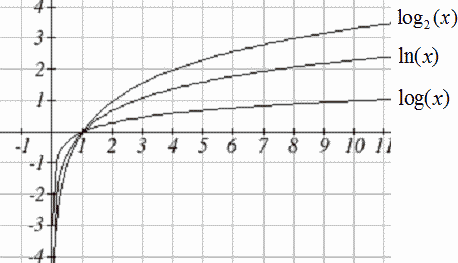
\includegraphics{images/image080.png}
\caption{}
\end{figure}

Another important observation made was the domain of the logarithm:
\textbackslash{}(x \textbackslash{}gt 0\textbackslash{}). Like the
reciprocal and square root functions, the logarithm has a restricted
domain which must be considered when finding the domain of a composition
involving a log.

\hypertarget{example-8}{%
\paragraph{Example 8}\label{example-8}}

Find the domain of the function \textbackslash{}(
f(x)=\textbackslash{}log(5-2x) \textbackslash{}).

The logarithm is only defined when the input is positive, so this
function will only be defined when \textbackslash{}( 5-2x
\textbackslash{}gt 0 \textbackslash{}). Solving this inequality,
\textbackslash{}( -2x \textbackslash{}gt -5 \textbackslash{}), so
\textbackslash{}( x\textbackslash{}lt \textbackslash{}frac\{5\}\{2\}
\textbackslash{}).

The domain of this function is \textbackslash{}( x\textbackslash{}lt
\textbackslash{}frac\{5\}\{2\} \textbackslash{}), or, in interval
notation, \textbackslash{}( \textbackslash{}left(-\textbackslash{}infty,
\textbackslash{}frac\{5\}\{2\} \textbackslash{}right) \textbackslash{}).

\begin{longtable}[]{@{}ll@{}}
\toprule
\endhead
\href{section1-7.php}{← Previous Section} &
\href{../chapter2/section2-1.php}{Next Section →}\tabularnewline
\bottomrule
\end{longtable}
